\chapter{Scheduler Queues} 
The pending events are managed by distinct scheduler queues that utilize different data structures to implement the 4 key operations (i.e. enqueue, peek dequeue, and cancel). We have compared the effectiveness of 7 different non-intrusive queue data structures namely: \ding{172} binary heap (\textbf{heap}), \ding{173} binomial heap (\textbf{binomHeap}), \ding{174} 2-tier heap (\textbf{2tHeap}), \ding{175} 2-tier Fibonacci heap
(\textbf{fibHeap}), \ding{176} 3-tier heap (\textbf{3tHeap}), \ding{177} Ladder Queue (\textbf{ladderQ}), and \ding{178} 2-tier Ladder Queue (\textbf{2tLadderQ}). The queues are broadly classified into two categories, namely: single-tier and multi-tier queues. Single-tier queues such as \textbf{heap} and \textbf{binomHeap} use only a single data structure for accomplishing the 4 key operations. Conversely, multi-tier queues organize events into tiers, with each tier implemented using different data structures. Table~\ref{tab:q-comp} summarizes the algorithmic time complexities of the 7 data structures discussed in the following subsections.

\begin{table}[!ht]\centering
\textbf{ \caption{Comparison of algorithmic time complexities of different
data structures}}\label{tab:q-comp}
\hspace{1cm}

Legend -- $l$: \#LPs, $e$: \#events / LP, $c$: \#concurrent events,

$z$: \#canceled events, \textsubscript{t2}\textit{k}: parameter, $1^{*}$: amortized constant

\begin{tabular}{lccc}
\toprule
Name & Enqueue & Dequeue & Cancel \\
\midrule
\textbf{heap}    & $\log(e\cdot l)$ & $\log(e\cdot l)$ & $z\cdot\log(e\cdot l)$ \\
\textbf{binomHeap}    & $\log(e\cdot l)$ & $\log(e\cdot l)$ & $z\cdot\log(e\cdot l)$ \\
\textbf{2tHeap}  & $\log(e) + $ & $\log(e) + $ & $z\cdot\log(e) + $ \\
& $\log(l)$ & $ \log(l)$      & $ \log(l)$ \\
\textbf{fibHeap} & $\log(e) + 1^{*}$ & $\log(e) + 1^{*}$ & $z\cdot\log(e) + 1^{*}$ \\
\textbf{3tHeap}  & $\log(\frac{e}{c}) + \log(l)$ & $\log(l)$ & $e + \log(l)$ \\
\textbf{ladderQ} & $1^{*}$ & $1^{*}$ & $e\cdot l$ \\
\textbf{2tLadderQ} & $1^{*}$ & $1^{*}$ & $e\cdot l \div$ \textsubscript{t2}\textit{k} \\
\bottomrule
\end{tabular}
\end{table}
\section{Binary Heap (heap)} 
The binary heap based (\textbf{heap}) is a commonly used data structure for implementing priority queues. It is a single tier-data structure and is implemented using a conventional array-based approach. A \textbf{std::vector} is used as the backing container and algorithms (\textbf{std::push\_heap}, \textbf{std::pop\_heap}) are used to maintain the heap. The heap is prioritized on both time stamp and LP's \emph{ID} (to dequeue batches of events), with the lowest time stamp at the root of the heap. Operations on the heap are logarithmic in time complexity -- given $l$ LPs each with $e$ events/LP, the time complexity of enqueue and dequeue operations is $\log(e\cdot l)$ as shown in Table~\ref{tab:q-comp}. If event cancellation requires $z$ events to be removed from the heap, the time complexity is $z\cdot \log(e\cdot l)$. Consequently, for long or cascading rollbacks the cancellation costs is high.

\section{Binomial Heap (binomHeap)} 
The \textbf{binomHeap} is another single-tier data structure that uses Binomial heap from the \textsc{boost} C++ library. In similarity to \textbf{heap}, \textbf{binomHeap} is prioritized on both time stamp and LP's \emph{ID}, with the lowest time stamped event at the root. Additionally, the operations on \textbf{binomHeap} are logarithmic with a time complexity for enqueue and dequeue operations of $\log(e\cdot l)$. A special property of Binomial heap is the ability to merge two heaps into a single heap with a time complexity of $\log(n)$. Given that \textbf{binomHeap} is a single-tier data structure and all of the LPs on an MPI-process share a PES queue, the merge operation is not relevant.

\begin{figure}[H] \centering
\begin{minipage}{0.55\linewidth}
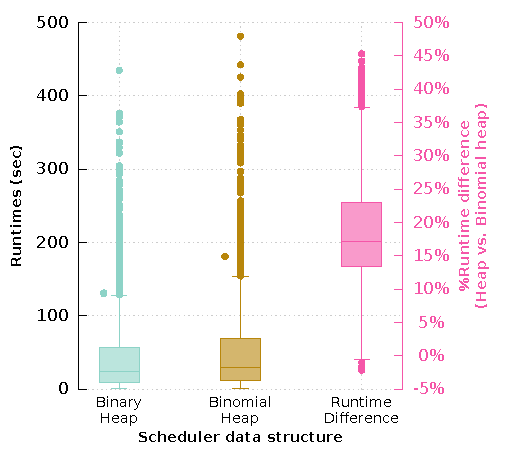
\includegraphics[width=\linewidth]{images/heap_binomHeap_compare.pdf}
\end{minipage}
\textbf{\caption{Comparison of heap and binomHeap execution time}}\label{fig:heapVbinomHeap}
\end{figure}

\subsection{Run time comparison of heap vs. binomHeap}
Due to similarities between Binary and Binomial Heap, we performed a comparison of \textbf{heap} and \textbf{binomHeap} to identify which one of the two data structures was the more effective priority queue based implementation of the PES queue. The comparison involved the production of serial run times for 2500 different configurations of PHOLD benchmark for both data structures. As shown in Figure~\ref{fig:heapVbinomHeap}, \textbf{heap} had a lower serial run time than \textbf{binomHeap}. The average run time for \textbf{heap} was 43.87 seconds and the average run time for \textbf{binomHeap} was 52.17 seconds. An unpaired two sample t-test was performed on the two sample run times to determine if averages were generally different. The data showed t-stat () > t-critical (1.96) and the p-value: 2.91E-315 << 0.05. Thus showing the averages were statistically different. A paired two sample t-test was also conducted and the paired t-test resulted in a p-value 2.01E-315
<< 0.05. Therefore, the null hypothesis (H0: difference between samples is zero) was rejected and we concluded that \textbf{heap} is generally faster than \textbf{binomHeap}. Based on the results, Binomial Heap was not used in any further implementation and assessment of the PES queue. 

\begin{figure}[H] \centering
\begin{minipage}{0.49\linewidth}
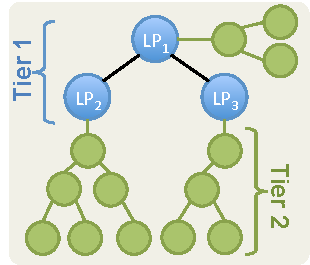
\includegraphics[width=\linewidth]{images/2tierQ}
\centerline{(a) 2-tier Heap}
\end{minipage}
\begin{minipage}{0.49\linewidth}
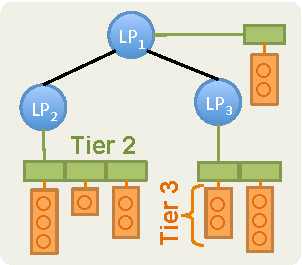
\includegraphics[width=\linewidth]{images/3tierQ}
\centerline{(b) 3-tier Heap}
\end{minipage}
\textbf{\caption{Structure of 2-tier \& 3-tier heap}}\label{fig:heaps}
\end{figure}

\section{Two-tier Heap (2tHeap)} 
The \textbf{2tHeap} is designed to reduce the time complexity of cancel operations by subdividing events into two distinct tiers as shown in Figure~\ref{fig:heaps}. The first tier has containers for each local LP on an MPI-process. Each of the tier-1 containers contain a heap of events to be processed by a given LP. In \textbf{2tHeap} both tiers are maintained as independent binary heaps. Consequently, given $l$ LPs and $e$ pending events per LP, enqueue and dequeue operates require
$\log e$ time to insert in tier-2 followed by $\log l$ time to reschedule the LP. Note that the tier-1 heap is updated only if the root event in tier-2 changes after an operation. Consequently, the best case time complexity becomes $\log e$ when compared to $\log e\cdot l$ for the \textbf{heap}. Furthermore, cancellation of events for an anti-message is restricted to just the tier-2 entries of LP \textsubscript{dest}  with utmost 1 tier-1 operation to update schedule position of LP \textsubscript{dest}. A \textbf{std::vector} is used as the backing storage for both tiers and standard algorithms are used to maintain the min-heap property for both tiers after each operation.

\section{2-tier Fibonacci Heap (fibHeap)} 
The \textbf{fibHeap} is an extension to the previous \textbf{2tHeap} data structure and uses a Fibonacci heap for scheduling LPs. The Fibonacci heap is a slightly modified version from the \textsc{boost} C++ library. The Fibonacci heap has an amortized constant time for changing key values and finding minimum. Consequently, we use it for the first tier which is responsible for scheduling LPs and use a standard binary heap for the second tier.  We do not use Fibonacci heap for the second tier because we found its runtime constants to be higher than a binary heap.  Accordingly, the time complexity for enqueue and dequeue operations is $\log(e) + 1^{*}$.

\section{Three-tier Heap (3tHeap)} 
The \textbf{3tHeap} builds upon \textbf{2tHeap} by further subdividing the second tier into two tiers as shown in Figure~\ref{fig:heaps}(b). The binary heap implementation for the first tier that manages LPs for scheduling has been retained from \textbf{2tHeap}. However, the 2nd tier is implemented as a list of containers sorted based on receive time of events. Each tier-2 container has a 3rd tier list of concurrent events. Assuming each LP has $c$ concurrent events on an average, there are $\frac{e}{c}$ tier-2 entries with each one having $c$ pending events. Inserting events in the \textbf{3tHeap} is accomplished via binary search at tier-2 with time complexity $\log\frac{e}{c}$ followed by an append to tier-3, a constant time operation. Enqueue to tier-2 is followed by an optional heap fix-up of time complexity $\log l$ as summarized in Table~\ref{tab:q-comp}. Dequeue operation for a LP removes a tier-2 entry in constant time followed by a $\log l$ heap fix-up for scheduling. Event cancellation has time complexity of $e + \log(l)$ as it requires inspecting each event in tier-3 followed by heap fix-up. As an implementation optimization, we recycle tier-2 containers to reduce allocation and deallocation overhead.

\begin{figure}[H] \centering
\begin{minipage}{0.49\linewidth}
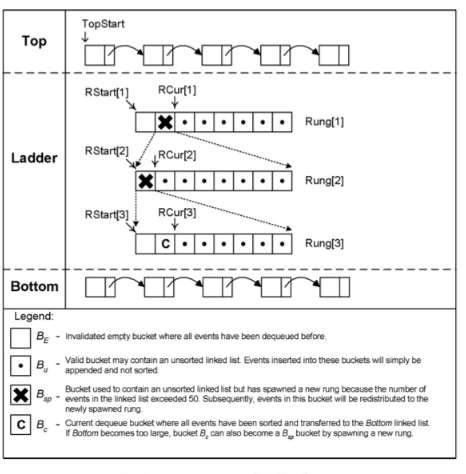
\includegraphics[width=\linewidth]{images/LadderQueue1.png}
\centerline{(a) Structure} \\

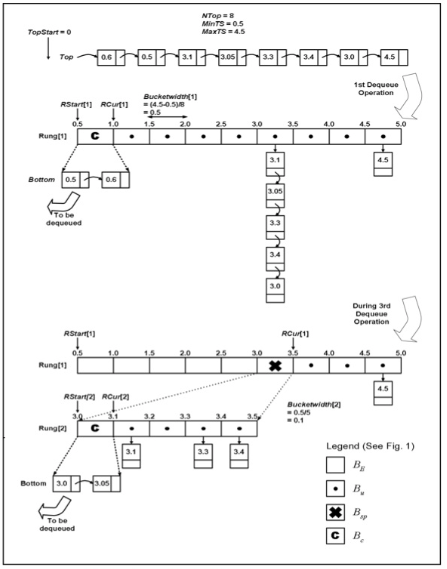
\includegraphics[width=\linewidth]{images/LadderQueue2.png}
\centerline{(b) Dequeue Operations}
\end{minipage}
\textbf{\caption{Structure of Ladder Queue} Source: Tang et al.~\cite{tang-05}}\label{fig:ladderQ}
\end{figure}

\section{Ladder Queue (ladderQ)} 
The \textbf{ladderQ} is a priority queue implementation proposed by Tang et al~\cite{tang-05} with amortized constant time complexity as summarized in Table~\ref{tab:q-comp}. Several investigators have independently verified that for sequential DES the \textbf{ladderQ} outperforms other priority queues, including: simple sorted list, binary heap, Splay tree, Calendar queue, and other multi-list data structures~\cite{dickman-13,franceschini-15,tang-05}. There are two key ideas underlying the Ladder Queue, namely: minimize the number of events to be sorted and delay sorting of events as much as possible. The multi-tier data structures also aim to minimize the number of events to be sorted. However, in contrast to the \textbf{ladderQ}, the other data structures always fix-up and maintain a minimum heap property. As shown in Figure~\ref{fig:ladderQ}(a), the ladder queue consists of the following 3 substructures:
\begin{enumerate}[leftmargin=*,topsep=0pt]
\item \emph{Top}: An unsorted list which contains events scheduled into the distant future or epoch.

\item \emph{Ladder}: Consists of multiple rungs, \textit{i.e.,}list of buckets. Each bucket contains list of events with a finite range of time stamp values. Hence, although events within a bucket are not sorted, the buckets on a rung are organized in a sorted order. The \textbf{ladderQ} minimizes the number of events to be finally sorted by recursively breaking large buckets into smaller buckets in lower rungs of its ladder. Lower rungs in the ladder have smaller buckets with smaller time ranges and the maximum number of rungs in Ladder is 8.

\item \emph{Bottom}: This substructure contains a sorted list of events to be processed. Inserts into \emph{Bottom} must preserve sorted order. Hence, the \textbf{ladderQ} strives to maintain a short bottom by moving events back into the ladder, as needed. The default threshold value at which events from Bottom are moved into Ladder is 50~\cite{tang-05}.\end{enumerate} 

At the beginning of a simulation, enqueue operations only involve the insertion of events into \emph{Top}. As the simulation progresses, the insertion of events can occur at any level of the data structure. The insertion of events in \emph{Top} and Ladder is an O(1) operation that involves adding events to a list that remains unsorted. The onset of dequeue operations involves moving unsorted events from \emph{Top} into a newly formed rung in Ladder. The time range or bucket-width of a rung is established by taking the difference between the highest and lowest time stamp and dividing the difference by the total number of events. As shown in Figure~\ref{fig:ladderQ}(b), the bucket-width computed from the time stamp in \emph{Top} is (4.5\textbf{max} - 0.5\textbf{min})/8 = 0.5. In accordance with their timestamps, events from \emph{Top} are placed into the appropriate buckets in Rung-1. Consequently, events with time stamps 0.5 and 0.6 are placed in the 1st bucket of Rung-1. In cases, where the number of events in a bucket exceeds the established threshold, a new rung is generated to store those events. For example, in Figure~\ref{fig:ladderQ}(b), Rung-2 is generated for time stamped events in the range of 3.0 to 3.5. As shown in the Figure, The bucket containing events are sequentially removed from the bottom most rung in Ladder. The events are inserted in sorted LTSF order into \emph{Bottom}, where events are dequeued for further processing. The clearing of events in Ladder and Bottom kickoffs the movement of additional events from \emph{Top} into the two lower substructures. The implementation of Ladder Queue in MUSE adheres to the functionality described in ~\cite{tang-05} with some modifications.   

\begin{figure}[H] \centering
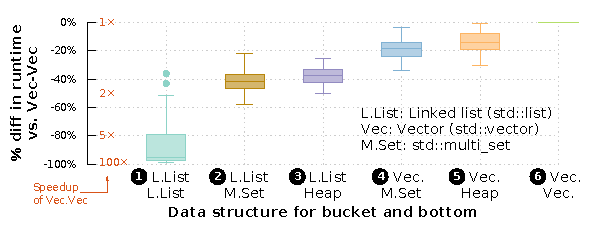
\includegraphics[width=\linewidth]{images/lq_config_compare}
\centerline{(a) Comparison sequential runtimes}
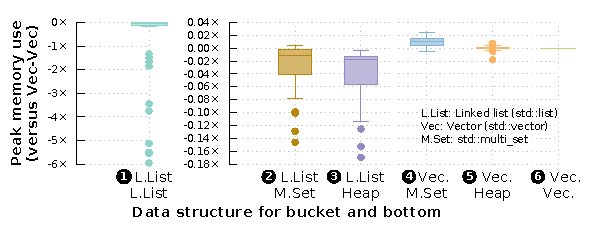
\includegraphics[width=\linewidth]{images/lq_config_memory_compare}
\centerline{(b) Peak memory used} 
\textbf{\caption{Comparison of execution time and peak memory for \textbf{PHOLD} benchmark (different parameter settings) using 6 different \textbf{ladderQ} configurations}}\label{fig:lq-configs}
\end{figure}

\subsection{Fine tuning Ladder Queue performance}\label{sec:fine-tune-lq}

As previously stated, our implementation closely followed the design in the original paper by Tang et al~\cite{tang-05}. However, to minimize runtime constants, we have explored different configurations for the buckets and the \emph{Bottom} in the \textbf{ladderQ}. Specifically, we have explored the
following 6 configurations -- \ding{182} \underline{L.List-L.List}: using a doubly-linked list (L.List) implemented by \textbf{std::list}) for buckets and bottom. Events are inserted into bottom via linear search as proposed by Tang et al. \ding{183} \underline{L.List-M.Set}: L.List for buckets and a Multi-set ($\log n$ operations) for bottom, \ding{184} \underline{L.List-Heap}: a L.List and a binary heap (backed by a \textbf{std::vector}) for bottom, \ding{185} \underline{Vec-M.Set}: a dynamically growing array (\textit{i.e.,} \textbf{std::vector}) for buckets and Multi-set bottom, \ding{186} \underline{Vec-Heap}: Vector buckets and binary heap for bottom, and \ding{187} \underline{Vec-Vec}: Vector for buckets and bottom. This configuration enables using quick sort(\textit{i.e.,} \textbf{std::sort}) for sorting buckets and binary search for inserting events into bottom.

Runtime comparison of the 6 \textbf{ladderQ} configurations is summarized in Figure~\ref{fig:lq-configs}. The data was obtained using \textbf{PHOLD} with different parameter settings. The \ding{187}$^{th}$ Vec-Vec configuration was the fastest and performance of other configurations are shown relative to it in Figure~\ref{fig:lq-configs}(a). The L.List-L.List configuration was generally the slowest and performed 85 \texttimes (or ~98\%) slower than the Vec-Vec configuration. The peak memory used for simulations is shown in Figure~\ref{fig:lq-configs}(b), in comparison with the Vec-Vec configuration.  As shown by the charts in Figure~\ref{fig:lq-configs}, the increased performance of Vec-Vec comes at about a 6\texttimes increase in peak memory footprint when compared to L.List-L.List configuration. This increased footprint arises because the \textbf{std::vector} internally doubles its capacity as it grows. With many buckets in the \textbf{ladderQ}, each implemented using a \textbf{std::vector}, the overall peak memory footprint is higher. Certainly, the increased capacity is used if the number of events in buckets grow. However, the Vec-M.Set and Vec-Heap configurations consume a bit more memory in some configurations, showing that Vec-Vec is not the worst in memory consumption. Consequently, we use the Vec-Vec configuration as it provides the fastest performance among the 6 configurations.

\begin{figure}[H]\centering
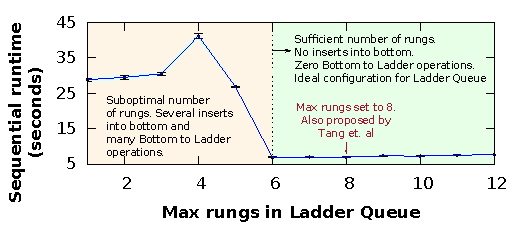
\includegraphics[width=\linewidth]{images/max_rung_effect}
\textbf{\caption{Impact of limiting rungs in Ladder}}\label{fig:max-rungs}
\end{figure}

The maximum number of rungs in the \emph{Ladder} also influences the overall performance of the \textbf{ladderQ}~\cite{tang-05}. The chart in Figure~\ref{fig:max-rungs} illustrates the impact of limiting the maximum number of rungs in the \textbf{ladderQ}. When the rungs are too few, the timestamp-based width of buckets is larger and more events with many different timestamps are packed into buckets. This also
causes the \emph{Bottom} to be longer with events spanning a broader range of timestamps. Consequently, when inserts happen into \emph{Bottom}, many \emph{Bottom}-to-\emph{Ladder} re-bucketing operations are triggered to ensure bottom is short. These re-bucketing operations with many events significantly degrade
performance. However, once sufficient number of rungs (6 rungs in this case) are permitted the events are better subdivide into smaller timestamp-based bucket widths. Small bucket widths in turn minimize
inserts into bottom and \emph{Bottom}-to-\emph{Ladder} operations, ensuring good performance.

The chart in Figure~\ref{fig:max-rungs} shows that a minimum of 6 rungs is required. For some select configurations of larger models we observed (data not shown) that 5 rungs would be sufficient. However, the number of rungs cannot exceed beyond a threshold to avoid infinite spawning of rungs~\cite{tang-05}.  Moreover, it limits the overheads involved in re-bucketing events from rung-to-rung~\cite{tang-05}. Accordingly, based on the observations in figure~\ref{fig:max-rungs}, we decided to adopt a maximum of 8 rungs, consistent with the threshold proposed by Tang et al~\cite{tang-05}. Furthermore, we trigger \emph{Bottom}-to-\emph{Ladder} re-bucketing only if the \emph{Bottom} has events at different timestamps to further reduce inefficiencies.

\subsection{Shortcoming of Ladder Queue for optimistic PDES}\label{sec:lq-prob}

The amortized constant time complexity of enqueue and dequeue operations enable the \textbf{ladderQ} to outperform other data structures in sequential simulations~\cite{dickman-13,franceschini-15,tang-05}.
However, canceling events, requires a linear scan of pending events because \emph{Top} and buckets in rungs are not sorted. In practice, scans of \emph{Top}, \emph{Ladder} rung buckets, and \emph{Bottom} can
be avoided based on cancellation times. Nevertheless, in a general case, event cancellation time complexity is proportional to the number of pending events -- \textit{i.e., } $e\cdot l$ as summarized in
Table~\ref{tab:q-comp}. This issue is exacerbated in large simulations where thousands of events are typically present in \emph{Top} and buckets in various rungs.

In this context, it is important to recollect from that -- as an optimization, \textbf{MUSE} utilizes only one anti-message to from LP \textsubscript{sender} to LP \textsubscript{dest} to cancel all $n$ events sent after $t_{rollback}$ (rather than sending $n$ individual anti-messages) which reduces overheads. Furthermore, with our centralized scheduler design, only events received from LPs on
other MPI-processes can trigger rollbacks. Consequently, the number of scans of the \textbf{ladderQ} that actually occur is significantly fewer in our case, despite the aggressive cancellation strategy.

\begin{figure}\centering
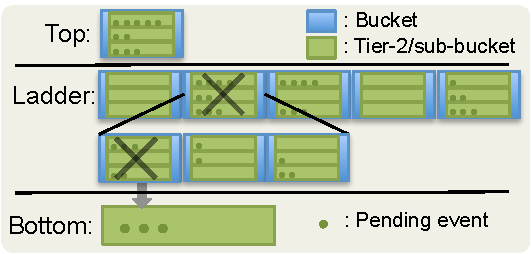
\includegraphics[width=\linewidth]{images/2tLadderQ}
\textbf{\caption{Structure of 2-tier Ladder Queue (\textbf{2tLadderQ}) with 3 sub-buckets / bucket (\textit{i.e.,} \textsubscript{t2} \textit{k}=3)}}\label{fig:2tLadderQ}
\end{figure}

\section{2-tier Ladder Queue (2tLadderQ)} \label{sec:2tLadderQ}

A key shortcoming of the Ladder Queue for Time Warp based optimistic PDES arises from the overhead of canceling events used for rollback recovery. Our experiments show that event cancellation overhead of \textbf{ladderQ} is a significant bottleneck in parallel simulation. On the other hand, our multi-tier data structures, where pending events are more organized, performed well.

Consequently, to reduce cost of event cancellation, we propose a 2-tier Ladder Queue (\textbf{2tLadderQ}) in which each bucket in \emph{Top} and \emph{Ladder} is further subdivided into \textsubscript{tk} sub-buckets, where \textsubscript{tk} is specified by the user. Figure~\ref{fig:2tLadderQ} illustrates an overview of the \textbf{2tLadderQ} with \textsubscript{tk} = 3 sub-buckets in each bucket. Given a bucket, a hash of the sending LP's ID (or the receiver LP ID, one or the other but not both) is used to locate a sub-bucket into which the event is appended. Currently, we use a straightforward LP \textsubscript{sender} modulo \textsubscript{tk} as the hash function. Consequently, enqueue involves just 1 extra modulo
instruction over regular \textbf{ladderQ} and hence retains its amortized constant time complexity. Similar to buckets, the sub-buckets are implemented using standard \textbf{std::vector} with events added or
removed only from the end to ensure amortized constant-time operation.

The dequeue operations for a bucket require iterating over each sub-bucket.  However, for a small, fixed value of \textsubscript{tk}, the overhead becomes an ammortized constant.  The constant overhead is determined by the value of \textsubscript{tk}. Consequently, dequeue also retains the amortized constant characteristic from regular \textbf{ladderQ} as summarized in Table~\ref{tab:q-comp}. Currently, we do not subdivide \emph{Bottom} but leave it as a possible future optimization.

\begin{figure}\centering
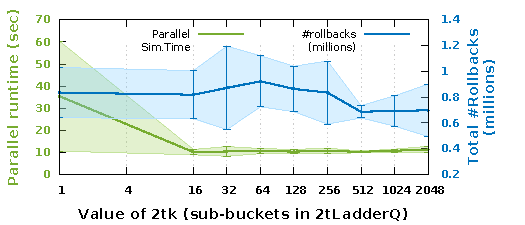
\includegraphics[width=\linewidth, height = 6cm]{images/2tlq_t2k_effect}
\textbf {\caption{Effect of varying \textbf{tk} }}\label{fig:2tk}
\end{figure}

\subsection{Performance gain of \textbf{2tLadderQ}}

The primary performance gain for \textbf{2tLadderQ} arises from the reduced time complexity for event cancellation. Since each bucket is sub-divided, only $1\div$\textsubscript{tk} fraction of events need to be checked during cancellation. For example, if \textsubscript{t2}\textit{k}=32, only $\frac{1}{32}$ of the pending events are scanned during cancellation. This significantly reduces the time constants in larger simulations enabling rapid rollback recovery.

The value of \textsubscript{t2}\textit{k} is a key parameter that influences the overall constants in \textbf{2tLadderQ}. For sequential simulation, where event cancellations do not occur, we recommend \textsubscript{t2}\textit{k}=1. With this setting the performance of \textbf{2tLadderQ} is very close to that of the regular \textbf{ladderQ}. However, in parallel simulation, the value of \textsubscript{t2}\textit{k} must be greater than 1 to realize benefits of its design. Figure~\ref{fig:2tk} shows the effect of changing the size of \textsubscript{t2}\textit{k} in a parallel simulation with 16 MPI processes. The total rollbacks in the simulations were with 10\% (except for \textsubscript{t2}\textit{k}=512, which for this model experienced fewer rollbacks). Nevertheless, for \textsubscript{t2}\textit{k}=1, the simulation has \emph{much} higher runtime due to event cancellation overheads.  The runtime dramatically decreases as \textsubscript{t2}\textit{k} is increased. The runtime remains comparable for a broad range of values, namely: 64$\le$\textsubscript{t2}\textit{k}\textless512. However, for \textsubscript{t2}\textit{k}$\ge$512, we noticed slow increase in runtime due to overhead of larger sub-buckets. Consequently, we have used a value of \textsubscript{t2}\textit{k}=128 for parallel simulation. We anticipate \textsubscript{t2}\textit{k} value to vary depending on the hardware configuration of the compute cluster used for parallel simulation. 


